\section{Budowa aplikacji}
\begin{figure}[H]
	\centering
	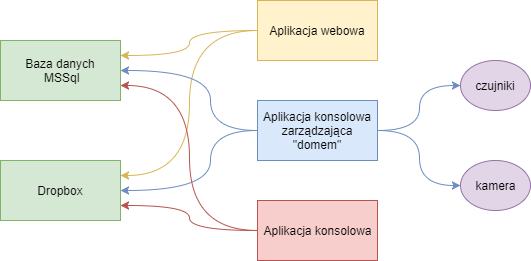
\includegraphics[scale=0.8]{schemat_systemu.png}
	\caption{Budowa systemu zarządzania domem}
	\label{fig:schemat_systemu}
\end{figure}
Aplikację powstałą na potrzeby tej pracy można podzielić na 3 moduły, które zostały przedstawione na rysunku \ref{fig:schemat_systemu}, a składają się na nie :
\begin{itemize}
\item Aplikacja webowa- interfejs pozwalający na zlecanie nowych zadań aplikacji konsolowej oraz odczyt wyników przesłanych przez nią oraz przez program zarządzający domem,
\item Aplikacja konsolowa- przetwarza zadania detekcji oraz rozpoznawania twarzy zlecone za pomocą aplikacji webowej,
\item Program zarządzający domem- przekazuje cyklicznie odczytywane dane z czujników oraz wykryte ruchy do bazy danych, w celu dalszej obróbki przez pozostałe moduły.
\end{itemize}
Na usługi pomocnicze wykorzystane w projekcie składają się
\begin{itemize}
\item baza danych- przechowywanie danych o dodanych zadaniach, wynikach, nauczonych sieciach neuronowych oraz osobach,
\item dropbox- przechowywanie większych plików- obrazów oraz nauczonych modeli sieci.
\end{itemize}